\documentclass{article}
\usepackage[utf8]{inputenc}
\usepackage{amsmath}
\usepackage{amsfonts}
\usepackage{amssymb}
\usepackage{graphicx}
\usepackage{geometry}
\usepackage{xcolor}

\newcommand{\inv}{^{-1}}   
\newcommand{\Z}{\mathbb Z}
\newcommand{\R}{\mathbb R}
\newcommand{\Q}{\mathbb Q}
\newcommand{\C}{\mathbb C}
\newcommand{\N}{\mathbb N}

\begin{document}
\pagecolor{black}
\color{white}

\noindent{\bf 1.}
\begin{align*}
    \frac{0.3\mu C}{1\mu s} &= 0.3 \frac Cs
\end{align*} Thus, the spark must contain $0.3$A of current.

\bigskip
\noindent{\bf 2.}
\begin{align*}
    4.5V &= .06A \cdot R \\
    75 \frac VA &= R
\end{align*} Thus, the bulb's resistance is $75 \Omega$.

\bigskip
\noindent{\bf 3.}
\begin{align*}
    \frac{1000 W}{115 V} &= 8.695652173913043A \\
\end{align*}
\begin{align*}
    115V &= 8.695652173913043A \cdot R \\
    13.225 \frac{V}{A} &= R
\end{align*} Thus, the toaster's resistance is $13.225\Omega$.

\bigskip
\noindent{\bf 4.}

    I would expect the stereo to use $4\Omega$ speakers, since they are quiet, so they're probably not doing a lot of work. Since $P= IV = I^2R$, increasing the resistance should increase the wattage of the speaker, and thus the rate at which it does work. That makes me think the speaker has a low resistance.

\bigskip
\noindent{\bf 5.}

    A 56k$\Omega$, 1\% resistor would have the following markings:

    Green, Blue, Orange, Pink.

\bigskip
\noindent{\bf 6.}

    $200\Omega$ resistors have the following markings:

    Red, Black, Brown.

    This is a problem, since when viewed upside-down, it would be Brown, Black, Red, which is the code for a 1000$\Omega$ resistor.

\bigskip
\noindent{\bf 7.}

    A 325Ah battery has a capacity of $325 \cdot 3600 = 1170000$C.

\bigskip
\noindent{\bf 8.}

    Largest: $1522.5\Omega$

    Smallest: $1377.5\Omega$

\bigskip
\noindent{\bf 9.}

    29463 is 111001100010111 in binary, and 7317 in hex.

\newpage
\noindent{\bf 10.}

\begin{center}
    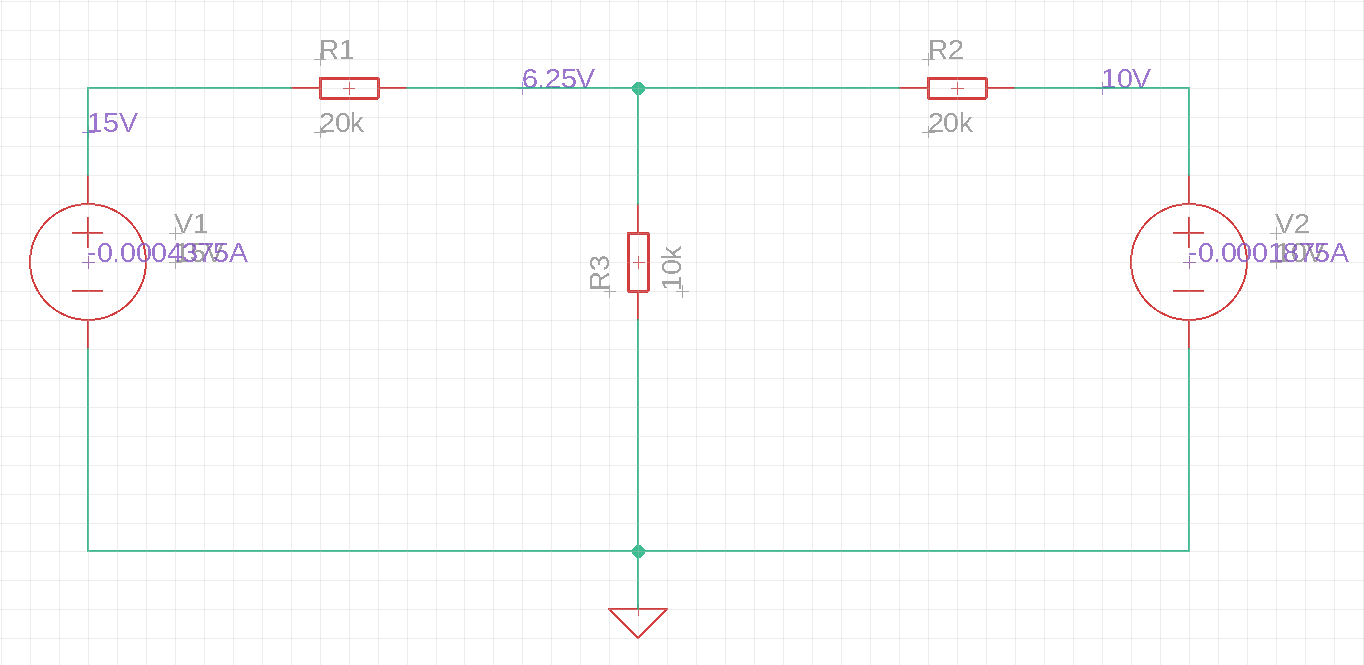
\includegraphics[scale=.5]{hw-1-eagle.png}
\end{center}

\end{document}
